\documentclass[14pt]{extarticle}
% \documentclass[14pt]{article}

% \usepackage[style=authoryear,maxbibnames=9,maxcitenames=2,uniquelist=false,backend=biber,doi=false,url=false]{biblatex}
% \addbibresource{$BIB} % bibtex location
% \renewcommand*{\nameyeardelim}{\addcomma\space} % have comma in parencite
\usepackage{natbib}

\usepackage{xcolor}
\usepackage{amsmath}
\newcommand{\tuple}[1]{ \langle #1 \rangle }
%\usepackage{automata}
\usepackage{times}
\usepackage{ltablex}
\usepackage{tasks}

%%%%%% Template
\usepackage{hyperref}
\hypersetup{colorlinks=true,allcolors=blue}

\usepackage{vmargin}
\setpapersize{USletter}
\setmarginsrb{1.0in}{1.0in}{1.0in}{0.6in}{0pt}{0pt}{0pt}{0.4in}

% HOW TO USE THE ABOVE:
%\setmarginsrb{leftmargin}{topmargin}{rightmargin}{bottommargin}{headheight}{headsep}{footheight}{footskip}
%\raggedbottom
% paragraphs indent & skip:
\parindent  0.3cm
\parskip    -0.01cm

\usepackage{tikz}
\usetikzlibrary{backgrounds}

% hyphenation:
% \hyphenpenalty=10000 % no hyphen
% \exhyphenpenalty=10000 % no hyphen
\sloppy

% notes-style paragraph spacing and indentation:
\usepackage{parskip}
\setlength{\parindent}{0cm}

% let derivations break across pages
\allowdisplaybreaks

\newcommand{\orange}[1]{\textcolor{orange}{#1}}
\newcommand{\blue}[1]{\textcolor{blue}{#1}}
\newcommand{\red}[1]{\textcolor{red}{#1}}
\newcommand{\freq}[1]{{\bf \sf F}(#1)}
\newcommand{\datafreq}[2]{{{\bf \sf F}_{#1}(#2)}}

\def\qqquad{\quad\qquad}
\def\qqqquad{\qquad\qquad}

%%%%%%%%%%%%%%%%%%%%%%%%%%%%%%%%%%%%%%%%%%%%%%%%%%%%%%%%%%%%%%%%%%%%%%%%%%%%%%%%
%%%%%%%%%%%%%%%%%%%%%%%%%%%%%%%%%%%%%%%%%%%%%%%%%%%%%%%%%%%%%%%%%%%%%%%%%%%%%%%%

% fill-in-blank question style, found in https://tex.stackexchange.com/a/505089

\usepackage{ifthen}
\usepackage{tocloft}
\usepackage{exercise}
% \usepackage{xcolor}

% Set the Show Answers Boolean
\newboolean{showAns}
\setboolean{showAns}{false}
\newcommand{\showAns}{\setboolean{showAns}{true}}

% The length of the Answer line
\newlength{\answerlength}
\newcommand{\anslen}[1]{\settowidth{\answerlength}{#1}}

% ans command that indicates space for an answer or shows the answer in red
\newcommand{\ans}[1]{\settowidth{\answerlength}{\hspace{2ex}#1\hspace{2ex}}%
    \ifthenelse{\boolean{showAns}}%
        {\textcolor{red}{\underline{\hspace{2ex}#1\hspace{2ex}}}}%
        {\underline{\hspace{\answerlength}}}}%

\newcommand{\details}[1]{\settowidth{\answerlength}{#1}%
    \ifthenelse{\boolean{showAns}}%
        {\\ \textcolor{blue}{#1}}%
        {}}%

% Formatting how multiple choices Questions are formated.
\settasks{label=(\Alph*), label-width=30pt}


% Some commands for the Exercise Question package
\renewcommand{\QuestionNB}{\Large\protect\textcircled{\small\bfseries\arabic{Question}}\ }
\renewcommand{\ExerciseHeader}{} %no header
\renewcommand{\QuestionBefore}{3ex} %Space above each Q
\setlength{\QuestionIndent}{8pt} % Indent after Q number


% To create the list of answers with tocloft...
\newcommand{\listanswername}{Answers}
\newlistof[Question]{answer}{Answers}{\listanswername}

% Creates a TOC for Answers
\newcounter{prevQ}
\newcommand{\answer}[1]{\refstepcounter{answer}%
\ans{#1}%
\ifnum\theQuestion=\theprevQ%
        \addcontentsline{Answers}{answer}{\protect\numberline{}#1}% don't include the Q number
        \else%
        \addcontentsline{Answers}{answer}{\protect\numberline{\theQuestion}#1}%
        \setcounter{prevQ}{\value{Question}}%
        \fi%
        }%

% \hyphenpenalty=10000 % no hyphen
% \exhyphenpenalty=10000 % no hyphen
\sloppy              % hyphen

\newcommand{\HRule}{\rule{\linewidth}{0.5mm}}
\newcommand{\Hrule}{\rule{\linewidth}{0.3mm}}

%tocloft formatting listofanswers
\renewcommand{\cftAnswerstitlefont}{\bfseries\large}
\renewcommand{\cftanswerdotsep}{\cftnodots}
\cftpagenumbersoff{answer}
\addtolength{\cftanswernumwidth}{10pt}

\makeatletter% since there's an at-sign (@) in the command name
\renewcommand{\@maketitle}{%
  \parindent=0pt% don't indent paragraphs in the title block
  \centering
  {\Large \bfseries\textsc{\@title}} \\
  \vspace{5pt}
  {\large \textit{\@author}} \\
  \HRule \\
  \vspace{1em}
}
\makeatother% resets the meaning of the at-sign (@)


\title{ECON 2002.01 Problem Set 3 }
\author{Unit 6 \\
  \vspace{5pt}
    Hui-Jun Chen}


%%%%%%%%%%%%%%%%%%%%%%%%%%%%%%%%%%%%%%%%%%%%%%%%%%%%%%%%%%%%%%%%%%%%%%%%%%%%%%%%
%%%%%%%%%%%%%%%%%%%%%%%%%%%%%%%%%%%%%%%%%%%%%%%%%%%%%%%%%%%%%%%%%%%%%%%%%%%%%%%%
\begin{document}

\maketitle

\showAns
\listofanswer

\begin{Exercise}

\Question
(OUP-U6-Q1) Which of the following statements is true?
\answer{B}
\begin{tasks}(1)
    \task An order given in a firm is a request for a job that can be rejected by the employee.
        \details{Under a wage labour contract, an employee accepts the authority of the employer over the use of his or her time while at work. In other words, an order given in a firm is a command.}
    \task In a market, prices motivate and constrain people’s actions, and are determined as a result of the actions of a large number of participants.
        \details{This is true. By contrast, in a firm, owners or the managers direct the activities of their employees.}
    \task
        Contracts for products sold in markets temporarily transfer authority over the product from the seller to the buyer.
        \details{
        Contracts for products sold in markets permanently transfer ownership of the good from the seller to the buyer. Contracts for labour temporarily transfer authority over an employee’s activities from the employee to the manager or owner.
        }
    \task
    Asymmetric information in a firm is the details about the asymmetry of authority within the firm.
        \details{
    Asymmetric information is the problem of the owners or managers not always knowing what their subordinates know or do. This results in not all of their directions or commands being necessarily carried out.
        }
\end{tasks}


\Question
(OUP-U6-Q2)
Which of the following statements is true?
\answer{C}
\begin{tasks}(1)
    \task
The managers are residual claimants of the firm's profits.
        \details{
The residual is whatever remains after revenues are used to pay managers, employees, suppliers, creditors, and taxes. The owners (the shareholders) are the residual claimants.
        }
    \task
The owners of a firm are the only individuals who hold the firm’s shares.
        \details{
Shareholders can be financial organisations (such as pension funds) as well as individuals, particularly for large corporations.
        }
    \task
	With the separation of ownership and control, decisions are made by managers while the benefits of the decisions accrue to the owners.
        \details{
This is true and results in a potential conflict of interest.
        }
    \task
	The separation of ownership and control has costs that almost always outweigh the benefits.
        \details{
If this is the case then firms would not separate ownership and control. The many benefits of separation include ease of raising capital and transfer of ownership, risk diversification for the owners, ability to employ specialists as managers, and limited liability.
        }
\end{tasks}

\Question
(OUP-U6-Q3)
Which of the following statements regarding employment contracts are correct?
\answer{C}
\begin{tasks}(1)
    \task
The firm is required to state exactly what it needs the employee to do in an employment contract.
        \details{
Due to unforeseen future events, the firm cannot possibly know exactly what it will need the employee to do at the time the contract is signed.
        }
    \task
	The firm needs to specify exactly how much effort employees are expected to put into their job.
        \details{
It is impractical or too costly for the firm to observe exactly how much effort each employee puts into their job.
        }
    \task
Employees’ effort levels cannot be the basis of an enforceable contract.
        \details{
This is true – for example, a restaurant owner cannot take an employee to a court to decide whether he can withhold wages because the waiter had not smiled often enough.
        }
    \task
Employment contracts are incomplete as they can only specify things that both the employees and the business owner care about.
        \details{
Employment contracts are incomplete as they cannot specify things that both the employees and the business owner care about: how hard and well the employee will work, and for how long the worker will stay.
        }
\end{tasks}




\Question (OUP-U6-Q8)
Thomas earns £12 per hour in his current job and works 36 hours a week. He loves his job and puts in his maximum effort with no disutility. In fact, Thomas earns extra utility worth £3 per hour from camaraderie, status, and enjoyment of the job. If he loses this job Thomas has two choices. Either he is able to be self-employed, which earns him £7 an hour for 36 hours a week of work but also gives him disutility equivalent to £2 per hour, or he can be unemployed and receive an unemployment benefit of £150 per week. Thomas is expected to be able to find another job similar to his current one in 24 weeks. Then:
\answer{D}
\begin{tasks}(1)
    \task
Thomas’s next best option is to be unemployed.
        \details{
By being self-employed he will receive a benefit of (7 – 2) × 36 = £180 per week. This is higher than the unemployment benefit of £150 per week.
        }
    \task
The employment rent per hour is £8.
        \details{
The employment rent is (12 + 3) – (7 – 2) = £10 per hour.
        }
    \task
Thomas’s employment rent is £9,360.
        \details{
The employment rent is (12 + 3) – (7 – 2) = £10 per hour for 36 hours a week over the expected unemployment duration of 24 weeks i.e. 10 × 36 × 24 = £8,640.
        }
    \task
If Thomas chooses the self-employment option then his loss of employment rent is £8,640.
        \details{
		The loss of employment rent is the rent between the current job and self-employment. This is (12 + 3) – (7 – 2) = £10 per hour for 36 hours a week over the expected unemployment duration of 24 weeks i.e. 10 × 36 × 24 = £8,640.
        }
\end{tasks}


\Question
(OUP-U6-Q13)
Consider isocost lines drawn on a graph with hourly wage on the horizontal axis and effort per hour on the vertical axis. Which of the following statements is correct?
\answer{D}
\begin{tasks}(1)
    \task
Isocost lines intersect the horizontal axis at the reservation wage.
        \details{
Isocost lines go through the origin (zero wage, zero cost).
        }
    \task
The slope of the isocost line is the employer’s marginal rate of transformation of higher wages into worker effort.
        \details{
The slope of the isocost lines is the employer’s marginal rate of substitution, which is the rate at which the employer is willing to increase wages to get higher effort.
        }
    \task
Steeper isocost lines represent higher cost per unit of effort.
        \details{
The slope of the isocost lines represents the units of effort per dollar of wage cost. Steeper isocosts therefore mean more units of effort per dollar of wage cost, or equivalently, a lower cost per unit of effort.
        }
    \task
For an isocost lines with a slope of 0.07, the cost of unit of effort is \$14.3.
        \details{
The slope of the isocost lines represents the units of effort per dollar of wage cost, which is the inverse of the cost per unit of effort. The latter is therefore 1/0.07 = \$14.3.
        }
\end{tasks}




\Question (OUP-U6-Q16)
The figure depicts the efficiency wage equilibrium of a worker and a firm. Based on this information, which of the following statements is correct?
\answer{A}

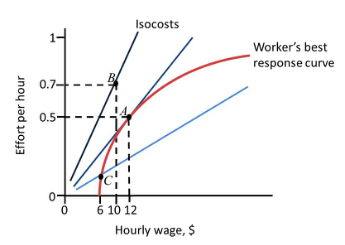
\includegraphics[width=\textwidth]{../QuestionBankImage/OUP-U6-Q15-01.png}
\begin{tasks}(1)
    \task
At A, given that the firm pays the hourly wage of \$12, the worker’s best response is to exert an effort of 0.5.
        \details{
This is true, by the definition of the worker’s best response curve.
        }
    \task
At A, given that the worker exerts an effort level of 0.5, the firm’s best response is to offer the hourly wage of \$12.
        \details{
The firm chooses to offer \$12 given the worker’s best response curve, rather than a particular effort level.	This is a sequential game where the firm chooses its action given the worker’s best responses to its actions.
        }
    \task
Therefore the worker receives no rent.
        \details{
The worker receives an employment rent because the efficiency wage is above her reservation wage. This wage level is required to induce her to put in some effort (of 0.5 in this case).
        }
    \task
The employer makes profits by coercing the worker to put in some effort.
        \details{
The employer’s power comes from the threat of job loss, which exists because the firm pays an efficiency wage above the worker’s reservation wage, giving the worker positive employment rents.
        }
\end{tasks}





\Question
(UCL-J15-Q3)
If unemployment benefits increase:
\answer{C}
\begin{tasks}(1)
    \task
A worker’s effort increases because the employment rent increases.
        \details{
The lost income relative to being employed falls, so the employment rent decreases and a worker’s effort decreases.
        }
    \task
Effort decreases because the disutility of effort decreases.
        \details{
Effort decreases because the employment rent decreases.
        }
    \task
The employment rent will fall unless the firm raises the wage.
        \details{The lost income relative to being employed falls, so the employment rent decreases, unless the firm increases the wage.}
    \task
The employment rent will increase unless the firm raises the wage.
        \details{The lost income relative to being employed falls, so the employment rent decreases, unless the firm increases the wage.}
\end{tasks}

\Question
(OUP-U6-Q19)
Consider a worker’s best response curve in the labour discipline model. Currently the firm chooses to pay £12 per hour to minimise the cost of effort, which induces an effort level of 0.6 from the worker. Now consider a rise in the unemployment benefit. Then:
\answer{C}
\begin{tasks}(1)
    \task
At the wage rate of £12 per hour the worker will now exert more than 0.6 of effort.
        \details{
As a result of the rise in the unemployment benefit, the best response curve shifts to the right. This reduces the effort induced for a given wage rate.
        }
    \task
The firm can lower the wage rate to below £12 to maintain the effort level of 0.6.
        \details{
As a result of the rise in the unemployment benefit, the best response curve shifts to the right. This means that the firm will have to pay more in order to induce the same level of effort.
        }
    \task
The firm’s new wage offer that minimises the cost of effort will be higher than £12.
        \details{
With the rightward shift in the best response curve, the point of tangency with the highest feasible isocost would shift to the right i.e. the firm will offer a higher equilibrium wage rate.
        }
    \task
The firm’s maximum units of effort per dollar of wage cost will be higher than before the rise in the unemployment benefit.
        \details{
With the rightward shift in the best response curve, the firm’s highest feasible isocost would be flatter i.e. the maximum units of effort per dollar of wage cost falls.
        }
\end{tasks}



\Question
(TEA-U6-Q2)
    Which of the following statements best describes the game played by the employer and the employee in the labour discipline model?
\answer{C}
\begin{tasks}(1)
    \task
The game is a simultaneous game in which the employer chooses the wage level and the employee chooses the effort level simultaneously.
        \details{
The game is a sequential game where the employer, knowing the employee’s possible decisions, selects the wage level first. The employee then selects his effort level given the offered wage level.
        }
    \task
The game is a one-off game in which the wage and effort levels are determined once and for all.
        \details{
The game is a repeated game where wages and effort levels decisions are made in each period.
        }
    \task
	The worker selects the effort level that balances his desire to keep his job with his desire to not exhaust himself on the job.
        \details{
    In the labour discipline model, putting in effort is costly for the worker, but he earns an employment rent from keeping his job. The amount of effort chosen depends on the relative size of these effects.
        }
    \task
The employer will attempt to maximise the firm’s profits by offering a wage equal to the worker’s reservation wage.
        \details{At his/her reservation wage, the worker will have no incentive to exert any effort. Therefore this will not be the firm’s optimal strategy.}
\end{tasks}


\Question (ECO-U6-Q5)
Maria earns \$12 per hour in her current job and works 35 hours a week. Her disutility of effort is equivalent to a cost of \$2 per hour of work. If she loses her job, she will receive unemployment benefit equivalent to \$6 per hour. Additionally, being unemployed has psychological and social costs equivalent to \$1 per hour. Then:
\answer{D}
\begin{tasks}(1)
    \task
The employment rent per hour is \$3.
        \details{
Employment rent per hour = wage – unemployment benefit – disutility of effort + disutility of unemployment = 12 – 6 – 2 + 1 = \$5. This is the net hourly benefit of being employed compared with unemployment.
        }
    \task
Maria’s reservation wage is \$6 per hour.
        \details{
Maria’s reservation wage = unemployment benefit – disutility of unemployment = 6 – 1 = \$5. This is the wage at which Maria is just willing to forgo her unemployment benefits for a job (but it is not enough to make her put in effort!).
        }
    \task
Maria’s employment rent if she can get another job with the same wage rate after 44 weeks of being unemployed is \$6,160.
        \details{
Maria’s employment rent = \$5 (employment rent per hour) × 35 hours per week × 44 weeks = \$7,700.
        }
    \task
Maria’s employment rent if she can only get a job at a lower wage rate after 44 weeks of being unemployed is more than \$7,700.
        \details{
If she could get a job at the same wage after 44 weeks, Maria’s employment rent = \$5 (employment rent per hour) × 35 hours per week × 44 weeks = \$7,700. If the new job would have a lower wage, her employment rent would be higher than \$7,700.
        }
\end{tasks}




\end{Exercise}

\end{document}
